\documentclass[11pt]{standalone}
\usepackage[usenames]{color} %used for font color
\usepackage{amssymb} %maths
\usepackage{amsmath} %maths

\usepackage[no-math]{fontspec}
\usepackage{unicode-math}
\setmainfont{Lato}
\setmathfont{Stix Two Math}

\usepackage{pgf,xcolor}
\definecolor{itwm_blue_04}{HTML}{005A94}
\definecolor{itwm_red}{HTML}{C00000}
\definecolor{itwm_yellow}{HTML}{FFEC7F}

\usepackage{tikz}
\usetikzlibrary{shapes.misc, shadows, decorations, arrows}
\usetikzlibrary{backgrounds}
\usetikzlibrary{calc}
\usepackage{pgfplots}
\pgfplotsset{compat=newest}
\usepgfplotslibrary{fillbetween}
\usepackage{tikzpagenodes}
\usetikzlibrary{patterns}

% 0,1 x 1,2
\begin{document}
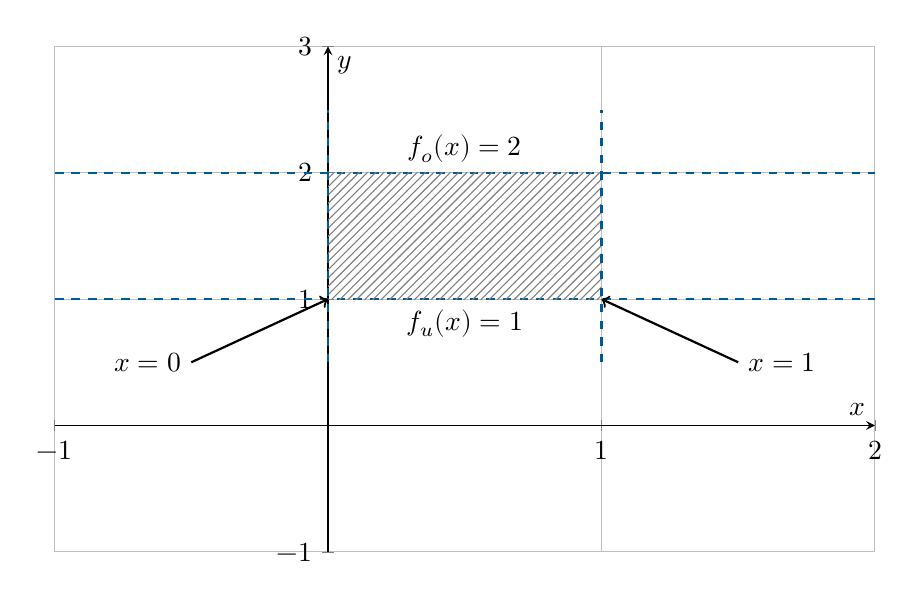
\begin{tikzpicture}
\begin{axis}[
    domain=-1:2,
    axis lines = center,
    xlabel = {$x$},
    ylabel = {$y$},
    height=8cm, width=12cm, 
    xmin=-1, xmax=2, ymin=-1, ymax=3, 
    xtick={-1, 0,...,2},
    ytick={-1, 0,...,3},
    grid = both
]
\addplot[draw=itwm_blue_04, dashed, samples=300, thick, name path=f]{2} node [pos=0.5, above] {$f_o(x)=2$};
\addplot[draw=itwm_blue_04, dashed, samples=300, thick, name path=f]{1} node [pos=0.5, below] {$f_u(x)=1$};
\fill [pattern=north east lines, pattern color=gray]  (0,1) rectangle (1,2);
\draw [draw=itwm_blue_04, dashed, thick] (0,0.5) -- (0 , 2.5); 
\draw [draw=itwm_blue_04, dashed, thick] (1,0.5) -- (1 , 2.5); 
\draw[->, thick] (-0.5,0.5)--(0,1) node[below, left, pos=0]{$x=0$};
\draw[->, thick] (1.5,0.5)--(1,1) node[below, right, pos=0]{$x=1$};
\end{axis}
\end{tikzpicture}
\end{document}